\documentclass[tikz,border=7pt]{standalone}

\usepackage{amsmath}
\usetikzlibrary{arrows.meta,positioning}

\definecolor{inputblue}{HTML}{4C78A8}
\definecolor{hiddenorange}{HTML}{F28E2B}
\definecolor{outputgreen}{HTML}{59A14F}
\definecolor{connectiongray}{HTML}{A7A7A7}

\begin{document}
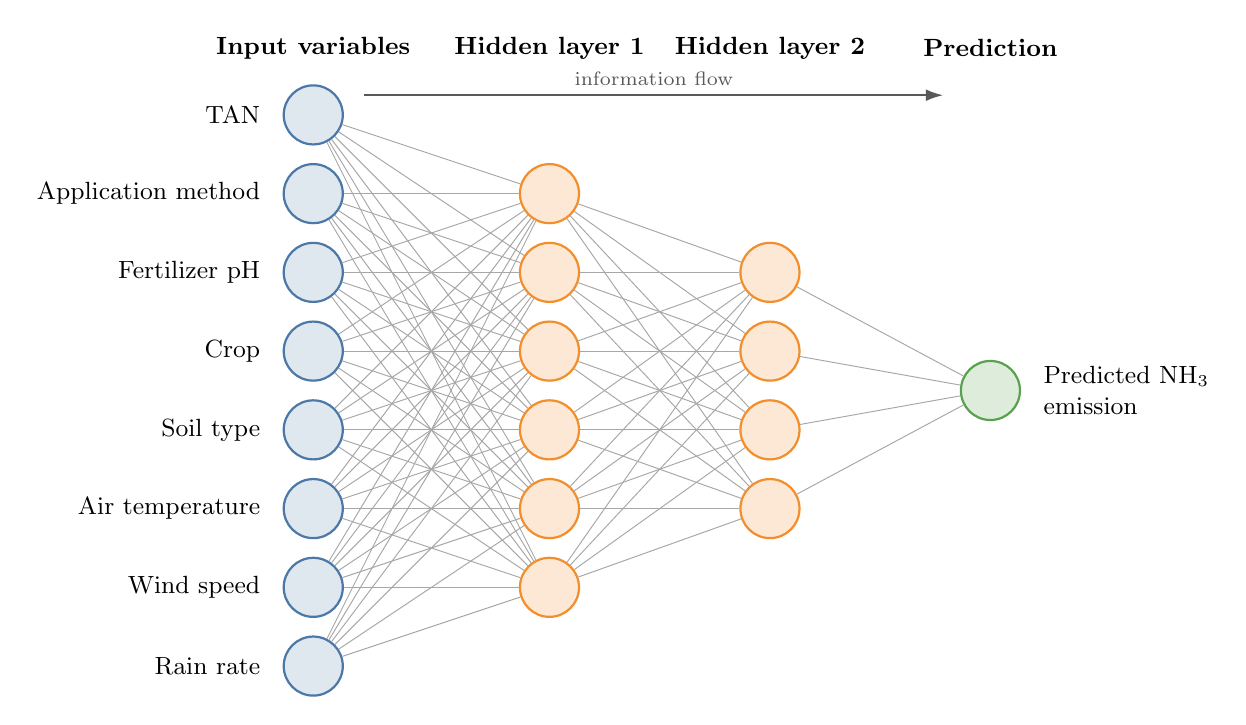
\begin{tikzpicture}[
  font=\small,
  neuron/.style={circle, draw, line width=0.8pt, minimum size=7.5mm,
                 inner sep=0pt},
  input neuron/.style={neuron, draw=inputblue, fill=inputblue!18},
  hidden neuron/.style={neuron, draw=hiddenorange, fill=hiddenorange!20},
  output neuron/.style={neuron, draw=outputgreen, fill=outputgreen!20},
  connection/.style={draw=connectiongray, line width=0.35pt},
  flow/.style={-{Latex[length=2.2mm,width=1.5mm]}, draw=black!65,
               line width=0.7pt},
  layer title/.style={font=\bfseries\small, align=center}
]

% Input variables
\foreach \name/\y [count=\i] in {
  {TAN}/3.50,
  {Application method}/2.50,
  {Fertilizer pH}/1.50,
  {Crop}/0.50,
  {Soil type}/-0.50,
  {Air temperature}/-1.50,
  {Wind speed}/-2.50,
  {Rain rate}/-3.50
}{
  \node[input neuron] (in-\i) at (0,\y) {};
  \node[anchor=east, align=right] at (-0.55,\y) {\name};
}

% Hidden layers
\foreach \y [count=\i] in {2.5,1.5,0.5,-0.5,-1.5,-2.5}
  \node[hidden neuron] (h1-\i) at (3.0,\y) {};

\foreach \y [count=\i] in {1.5,0.5,-0.5,-1.5}
  \node[hidden neuron] (h2-\i) at (5.8,\y) {};

% Output
\node[output neuron] (out) at (8.6,0) {};
\node[anchor=west, align=left] at (9.15,0)
  {Predicted NH$_3$\\emission};

% Fully connected successive layers
\foreach \i in {1,...,8}
  \foreach \j in {1,...,6}
    \draw[connection] (in-\i) -- (h1-\j);

\foreach \i in {1,...,6}
  \foreach \j in {1,...,4}
    \draw[connection] (h1-\i) -- (h2-\j);

\foreach \i in {1,...,4}
  \draw[connection] (h2-\i) -- (out);

% Layer labels and direction of information flow
\node[layer title] at (0,4.35) {Input variables};
\node[layer title] at (3.0,4.35) {Hidden layer 1};
\node[layer title] at (5.8,4.35) {Hidden layer 2};
\node[layer title] at (8.6,4.35) {Prediction};

\draw[flow] (0.65,3.75) -- node[above, font=\scriptsize,
  text=black!65] {information flow} (8.0,3.75);

\end{tikzpicture}
\end{document}

